\documentclass[conference]{IEEEtran}
\IEEEoverridecommandlockouts
\usepackage{cite}
\usepackage{amsmath,amssymb,amsfonts}
\usepackage{algorithmic}
\usepackage{graphicx}
\usepackage{textcomp}
\usepackage{xcolor}
\usepackage{listings}
\usepackage{booktabs}
\usepackage{adjustbox}
\usepackage{booktabs}   
\usepackage{placeins}   
\usepackage{float}       % For [H] positioning if needed
\usepackage{booktabs}  % For \toprule, \midrule, \bottomrule
\usepackage{tabularx}  % For adjustable width tables

\lstset{breaklines=true, basicstyle=\scriptsize\ttfamily, columns=fullflexible}
\def\BibTeX{{\rm B\kern-.05em{\sc i\kern-.025em b}\kern-.08em
    T\kern-.1667em\lower.7ex\hbox{E}\kern-.125emX}}
\begin{document}

\title{Graph-Based Machine Learning for Bibliographic Data Analysis: Node Classification and Link Prediction}

\author{\IEEEauthorblockN{Breeha Qasim, Ashbah Faisal \& Namel Shahid}
\IEEEauthorblockA{Department of Computer Science\\
Habib University\\
Karachi, Pakistan}}

\maketitle

\begin{abstract}
The application of graph-based machine learning algorithms to the analysis of bibliographic data is thoroughly examined in this research.  We investigate two fundamental tasks: link prediction to predict future collaborations and node classification to determine author domains.  Our approach builds and analyses a rich bibliographic network by combining machine learning frameworks with the Neo4j graph database.  In addition to offering insights into research collaboration patterns and domain classification, the study shows how well graph-based techniques capture complicated linkages seen in academic literature.
\end{abstract}

\section{Introduction}
\noindent Analysing bibliographic data has grown in significance for comprehending patterns of collaboration, research trends, and information sharing.  In this study, node classification and link prediction tasks are especially addressed by utilising graph-based machine learning approaches to analyse bibliographic data.  Using a large dataset sourced from bibliographic records, the study seeks to shed light on domain classification and academic collaboration trends.

\section{Methodology}
\subsection{Data Preprocessing}
\noindent The dataset consists of multiple CSV files containing information about authors, papers, journals, topics, and their relationships. The preprocessing pipeline, implemented in Python using Pandas, includes the following steps:

\begin{itemize}
    \item \textbf{Data normalization:} Converting column names to snake case and removing special characters
    \item \textbf{String cleaning:} Trimming whitespace and normalizing empty strings to None values
    \item \textbf{Duplicate removal:} Eliminating duplicate rows and rows with null primary keys 
    \item \textbf{ID mapping:} Creating integer IDs for authors, papers, and topics for efficient graph construction
    \item \textbf{Type conversion:} Converting numeric fields (year, citation count, volume) to nullable integers
\end{itemize}

\noindent The preprocessing pipeline handles seven main data files:
\begin{itemize}
    \item \texttt{author.csv}: Author information (ID, name, URL)
    \item \texttt{topic.csv}: Research topic information (ID, name, URL)
    \item \texttt{journal.csv}: Journal details (name, publisher)
    \item \texttt{paper.csv}: Paper metadata (ID, DOI, title, year, citations, etc.)
    \item \texttt{author\_paper.csv}: Author-paper relationships
    \item \texttt{paper\_topic.csv}: Paper-topic relationships
    \item \texttt{paper\_reference.csv}: Citation relationships between papers
\end{itemize}

% Data Cleaning Table

Table~\ref{tab:datacleaning} summarizes the number of rows and columns before and after cleaning for each file. 

\begin{table}[ht]
\centering
\caption{Dataset Statistics Before and After Cleaning}
\label{tab:datacleaning}
\begin{tabular}{|l|c|c|c|c|}
\hline
\textbf{File} & \textbf{Raw Rows} & \textbf{Raw Cols} & \textbf{Cleaned Rows} & \textbf{Cleaned Cols} \\
\hline
authors        & 38925  & 3 & 38925   & 4 \\
topics         & 6489   & 3 & 6489    & 4 \\
journals       & 165    & 2 & 51      & 2 \\
papers         & 693624 & 9 & 693624  & 10 \\
author\_paper   & 56450  & 2 & 56450   & 2 \\
paper\_topic    & 41880  & 2 & 41880   & 2 \\
paper\_journal  & 32647  & 3 & 32647   & 3 \\
paper\_reference& 1132044& 2 & 1132044 & 4 \\
\hline
\end{tabular}
\end{table}

\subsection{Graph Construction}
\noindent The bibliographic graph is constructed using Neo4j, with the following node types and their key attributes:

\begin{itemize}
    \item Author: \{author\_id, name, url\}
    \item Paper: \{paper\_id, doi, title, year, citation\_count, field, volume, date, url\}
    \item Journal: \{journal\_name, publisher\}
    \item Topic: \{topic\_id, name, url\}
\end{itemize}
The model comprises \texttt{739,089} nodes.
\noindent The graph structure also includes the following relationships:
\begin{itemize}
    \item $(\text{:Author})-[\text{:WROTE}] \xrightarrow{} (\text{:Paper})$: Authorship relationships
    \item $(\text{:Paper})-[\text{:PUBLISHED\_IN}] \xrightarrow{} (\text{:Journal})$: Publication venue
    \item $(\text{:Paper})-[\text{:HAS\_TOPIC}] \xrightarrow{} (\text{:Topic})$: Research topic classification
    \item $(\text{:Paper})-[\text{:CITES}] \xrightarrow{} (\text{:Paper})$: Citation network
\end{itemize}
The model also comprises \texttt{126,3011} relationships.

\noindent Figure~\ref{fig:graphmodel} illustrates the overall graph schema used in this project.

\begin{figure}[ht]
    \centering
    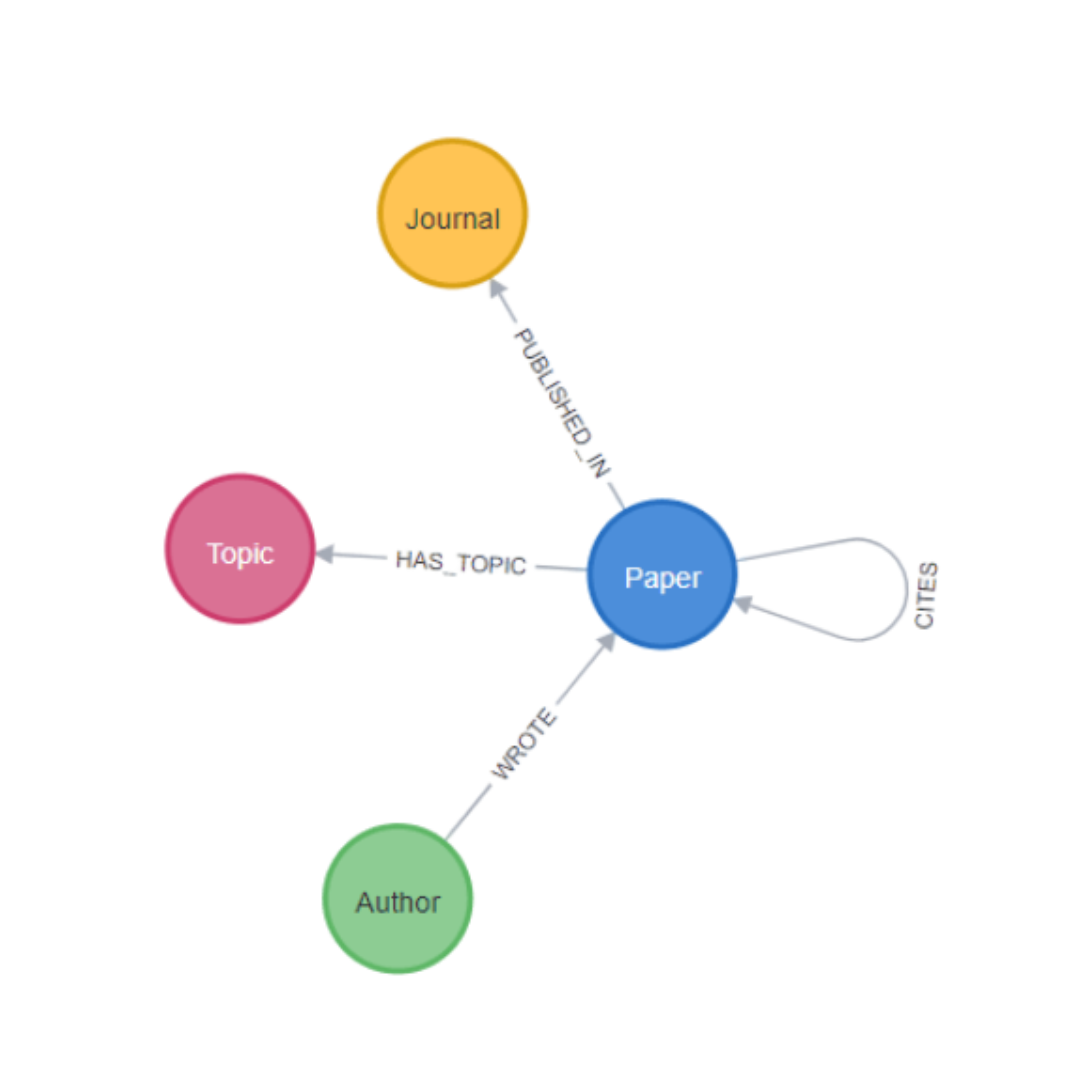
\includegraphics[width=0.48\textwidth]{Untitled design.png}
    \caption{Bibliographic Graph Model Schema}
    \label{fig:graphmodel}
\end{figure}

% Add rationale below the figure
\noindent By handling missing values, eliminating duplicates, normalising column names, and mapping IDs for effective graph creation, the preprocessing pipeline guarantees data consistency.  These Python-based procedures are crucial for creating a dependable and clean dataset for graph loading.

\noindent Unique constraints and indexes are built into Neo4j to ensure data integrity and speed up queries on important properties like names and IDs.  When importing millions of records, the use of \texttt{CALL IN TRANSACTIONS} allows for the effective bulk loading of huge CSV files, reducing memory utilisation and preventing transaction timeouts.

\noindent This method guarantees the accuracy and performance of the final graph database, facilitating operations related to machine learning and downstream analysis.

\noindent Since we only focused on the author-paper-co-authorship topology and did not model "year" or other temporal fields as distinct nodes, considering year as a straightforward relationship attribute proved adequate for the author/domain and future-collaboration use cases.
\noindent The graph construction process includes:
\begin{itemize}
    \item Creating unique constraints for primary keys
    \item Establishing indexes for frequently queried fields (paper year, author name)
    \item Batch loading of nodes and relationships in transactions
    \item Handling of missing and null values during node creation
\end{itemize}

\subsection{Node Classification (Author Classification)}
\noindent The node classification task focuses on \emph{Author Classification:} predicting the research domain or expertise of an author based on their co-authorship network.
\newline \newline
\noindent \textbf{\newline Preprocessing and Feature Engineering:}
\newline
A co-authorship network is constructed by creating \texttt{CO\_AUTHOR\_WITH} relationships between authors who have co-written papers. Around \texttt{44520} relationships were created. The label \texttt{author\_domain} was applied to each author around \texttt{12744} properties, indicating the dominating research topic (the most common topic among their works). Since Neo4j GDS does not support string labels, each unique domain is mapped to a numeric \texttt{domain\_id}. The training set (marked as \texttt{:TrainAuthor}) only contains authors with a known domain (\texttt{domain\_id IS NOT NULL}).

\noindent \textbf{\newline Modeling Approach:}
\newline
We implemented three RandomForest variants:
      \begin{enumerate}
        \item \emph{fastRP + domain\_id} only.
        \item \emph{fastRP + communityId + domain\_id}.
        \item \emph{fastRP + communityId + pageRank + domain\_id}.
      \end{enumerate}
Node features are generated via fastRP graph embeddings (capture local and global structure), Louvain community IDs (meso‐scale clusters), and PageRank scores (centrality). Due to long training times on the full dataset, we reduced:
      \begin{itemize}
        \item \texttt{embeddingDimension} from 128 \(\to\) 64  
        \item \texttt{numberOfDecisionTrees} from 50 \(\to\) 25  
      \end{itemize}
 We train with 4‑fold cross‑validation and a 25\% test split. Evaluation metrics: \texttt{accuracy, weighted F1‑score, and out‑of‑bag error}.

\noindent \textbf{\newline Assumptions and Rationale:}
\newline
The position and relationships of an author's co-author graph might be used to determine their research area.  The Louvain community identifies authors who share structural similarities and frequently discuss comparable subjects.  Node centrality serves as an extra predictive signal when PageRank is included.
% We attempted to use node regression (to predict domain directly as a continuous label), but the installed GDS version (1.6.1) does not support the \texttt{gds.beta.pipeline.nodeRegression.*} procedures.


\subsection{Link Prediction (Future Collaboration)}
\noindent By identifying trends in their current co-authorship network, the link prediction challenge seeks to anticipate which pairs of researchers will work together in the future.
\newline \newline
\noindent\textbf{Preprocessing and Feature Engineering:}\\
We begin by constructing an undirected co‐author graph in Neo4j, for every pair of authors who co‐wrote a paper, we merge a \texttt{CO\_AUTHOR\_WITH} relationship, carrying two edge properties:
    \begin{itemize}
      \item \texttt{year}: the publication year of at least one shared paper,  
      \item \texttt{sharedTopics}: the list of overlapping topics between their papers.
    \end{itemize}
After loading all such relationships, the in‐memory projection \texttt{predictionGraph} contains \texttt{38\,925} author nodes and \texttt{46\,116} edges. We then compute the following \emph{node‐level} features:
    \begin{itemize}
      \item \textbf{fastRP embeddings} (capture both local neighborhood and global position):
        \begin{itemize}
          \item \emph{128 dimensions} for Random Forest pipelines,  
          \item \emph{56 dimensions} for the Logistic Regression baseline,  
          \item \texttt{randomSeed}=42.
        \end{itemize}
      \item \textbf{degree} (number of collaborators) and its Min–Max scaled version, to encode each author’s collaboration activity.
    \end{itemize}
In addition, for some variants we compute:
    \begin{itemize}
      \item \texttt{Louvain communityId} to capture meso‐scale clusters of closely‐connected authors;  
      \item \texttt{PageRank} centrality and \texttt{triangleCount} (and scaled versions) to measure author prominence and local group cohesion.
    \end{itemize}
The main \emph{edge feature} in all pipelines is the \texttt{HADAMARD} product of node embeddings; the "RF + PageRank" variant additionally adds \texttt{COSINE} and \texttt{L2} similarities of embeddings, while the "Time‐based Hadamard" variant limits edges to those with valid \texttt{year} and \texttt{sharedTopics}.  We divide 70\% of the current edges for training, 20\% for testing, and reserve 10\% for validation (using five-fold cross-validation).  In order to balance positive cases, a 1:1 negative sampling ratio creates non-edges.
\newline \newline
\noindent\textbf{Modeling Approach:}\\
We compare five distinct pipelines in the GDS link‐prediction framework:
\newline \newline
\noindent \textbf{1. Logistic Regression (LR) Baseline \newline} 
Makes use of raw and scaled degrees + Hadamard product + fastRP embeddings (dimension 56) + split by 70 \% for train and 20 \% for test.
\newline \newline
\noindent \textbf{2. RandomForest (RF) Baseline \newline}  
The same features as LR,embedding dimension increased to 128, but with a RandomForest ensemble of 25 trees.  
Shows how switching to a non-linear, tree-based classifier using embedding-derived link characteristics improves performance.
\newline \newline
\noindent \textbf{3. RF + CommunityID \newline}  
Adds each node's participation in the Louvain community to the RF baseline features.  
 The hypothesis posits that there is a much higher likelihood of collaboration among writers who belong to the same community, such as departmental or subject clusters.
\newline \newline
\noindent \textbf{4. RF + PageRank \newline} 
Time-based splitting when all years are counted in train set except for 2020.
Adds PageRank centrality and (scaled) triangle counts, as well as Cosine and L2 embedding similarity, to the baseline.  
 Rationale: Authors in tightly-clustered neighbourhoods and central, well-connected authors may be more likely to form new partnerships; combining these orthogonal signals should enhance the quality of the ranking.
\newline \newline
\noindent \textbf{5. RF + Time‐based Hadamard \newline} 
The feature set is changed to Hadamard embedding + scaled degree. The RF baseline is used after filtering to only those edges with valid topical (\texttt{sharedTopics}) and temporal (\texttt{year}) annotations.  
 Motivation: By limiting the model to well-annotated edges, the model is focused on the most informative signals(same as for page rank).

\noindent All RandomForest variants use 25–50 trees (down from 100 in initial experiments to reduce training time), while LR remains a fast baseline.  
\newline \newline 
\noindent\textbf{Evaluation Metrics:}\\
We assess each model on
\begin{itemize}
  \item \texttt{AUPR/AUCPRs} (area under the precision–recall curve) on held‐out test edges,  
  \item \texttt{Out‐Of‐Bag (OOB) error} for RandomForest variants,  
  \item \texttt{Validation AUPRs} from 5‐fold cross‐validation.
\end{itemize}

\noindent\textbf{\newline Assumptions and Rationale:}
\begin{itemize}
  \item Structural embeddings (fastRP) summarize the graph neighborhood patterns that underlie collaboration.  
  \item Community detection groups authors by latent topical or institutional affiliation.  
  \item Centrality measures (PageRank) and local clustering (triangle counts) capture different aspects of author influence and cohesion.  
  \item Temporal and topical annotations on edges allow the model to learn recency and subject‐matching effects.  
  \item Comparing five variants quantifies the incremental benefit of each feature class, guiding future feature engineering in bibliographic link prediction.  
\end{itemize}


\section{Results}
\subsection{Node Classification Performance}

\noindent We compare three RandomForest variants on the author‐domain task:

\begin{table}[htbp]
  \centering
  \begin{tabularx}{\linewidth}{lXXXX}
    \toprule
    \textbf{Model} & \textbf{Test Accuracy} & \textbf{Test F1} & \textbf{Test OOB} & \textbf{Validation} \\
    \midrule
    fastRP + domain\_id & 0.5399 & 0.5032 & 0.5464 & 0.4995 \\
    fastRP + communityId & 0.5588 & 0.5295 & 0.5367 & 0.5142 \\
    \quad + domain\_id & & & & \\
    fastRP + communityId & 0.5599 & 0.5254 & 0.5287 & 0.5135 \\
    \quad + pageRank + domain\_id & & & & \\
    \bottomrule
  \end{tabularx}
  \vspace{0.3cm}
  \caption{Performance of RF classifiers with different feature sets (embeddingDimension=64, \#trees=25).}
  \label{tab:performance}
\end{table}


\subsection{Link Prediction Performance}

% \subsubsection{RF + CommunityId}
\begin{table}[H]
\centering
\begin{tabular}{lrrr}
\toprule
\textbf{Model} & \textbf{Test AUPR} & \textbf{Test OOB} & \textbf{Validation} \\
\midrule
RF + CommunityId & 0.6872 & 0.4981 & 0.6849 \\
\bottomrule
\end{tabular}
\vspace{0.3cm}
\caption{Table III: RF + CommunityId Performance}
\end{table}

% \subsubsection{Other Variants}
% \begin{table}[H]
% \centering
% \small
% \begin{tabular}{@{}lrrrr@{}}
% \toprule
% \textbf{Model} & \textbf{Avg} & \textbf{Outer} & \textbf{Test} & \textbf{Validation} \\
%  & \textbf{Train} & \textbf{Train} & \textbf{Score} & \textbf{Scores} \\
% \midrule
% RF + Time-Hadamard & 0.6966 & 0.6984 & 0.6860 & 0.6866 \\
% RF + PageRank & 0.9559 & 0.9436 & 0.9411 & 0.9107 \\
% Random Forest & 0.7319 & 0.7292 & 0.7254 & 0.7091 \\
% Logistic Regression & 0.8283 & 0.8283 & 0.8301 & 0.8283 \\

% % RF + Time-Hadamard & 0.6966 & 0.6984 & 0.6860 & 0.6866 \\
% \bottomrule
% \end{tabular}
% \vspace{0.3cm}
% \caption{Table IV: Other Model Variants Performance}
% \end{table}
\begin{table}[H]
\centering
\small
\begin{tabular}{@{}lrrrr@{}}
\toprule
\textbf{Model} & \textbf{Avg} & \textbf{Outer} & \textbf{Test} & \textbf{Validation} \\
 & \textbf{Train} & \textbf{Train} & \textbf{Score} & \textbf{Scores} \\
\midrule
RF + Time-Hadamard & 0.6966 & 0.6984 & 0.6860 & 0.6866 \\
RF + PageRank & 0.9559 & 0.9436 & 0.9411 & 0.9107 \\
\bottomrule
\end{tabular}
\vspace{0.3cm}
\caption{Table IV(a): Graph Feature Model Variants Performance}
\end{table}
\begin{table}[H]
\centering
\small
\begin{tabular}{@{}lrrrr@{}}
\toprule
\textbf{Model} & \textbf{Avg} & \textbf{Outer} & \textbf{Test} & \textbf{Validation} \\
 & \textbf{Train} & \textbf{Train} & \textbf{Score} & \textbf{Scores} \\
\midrule
Random Forest & 0.7319 & 0.7292 & 0.7254 & 0.7091 \\
Logistic Regression & 0.8283 & 0.8283 & 0.8301 & 0.8283 \\
\bottomrule
\end{tabular}
\vspace{0.3cm}
\caption{Table IV(b): Baseline Model Performance}
\end{table}

\section{Discussion}
\subsection{Key Findings}

\subsubsection{\textbf{Community Detection (Louvain)}}
With nearly perfect modularity (0.9914), the Louvain partitioning results show a hyper-fragmented cooperation network with remarkably robust, segregated communities.  While the greatest outlier (446 authors) suggests a rare, large-scale research hub, almost 17,000 little clusters (mean size: 2.23 authors) predominate, indicating that most collaborations are temporary or restricted to pairs.  This excessive localisation suggests highly specialised, insular teamwork with little interaction between communities, which may be a reflection of biases particular to a dataset or disciplinary barriers.  The 95th percentile cap of five writers emphasises even more how rare long-term group collaborations outside of tiny teams are.

\begin{table}[htbp]  % Added htbp placement specifier
  \centering
  \begin{tabular}{lr}
    \toprule
    \textbf{Metric}                     & \textbf{Value}   \\
    \midrule
    Modularity                          & 0.9914           \\
    Number of communities               & 17{,}432         \\
    Mean community size                 & 2.23 authors     \\
    Maximum community size              & 446 authors      \\
    Minimum community size              & 1 author         \\
    95th percentile community size      & 5 authors        \\
    \bottomrule
  \end{tabular}
  \vspace{0.3cm}
  \caption{Summary statistics of Louvain communities in the co-author graph.}
  \label{tab:louvain}
\end{table}

\subsubsection{\textbf{PageRank Centrality}}
With the majority of writers scoring close to the median (0.9741) and a small elite (top 1\% $>$ 2.2703) controlling network centrality, the PageRank study shows a highly skewed influence distribution.  A weakly linked core, with a few high-impact hubs bridging disparate communities, is suggested by the algorithm's inability to converge after 50 iterations.  This structure shows the "rich-get-richer" dynamics that are common in academic networks, where peripheral contributors (min: 0.15) stay isolated while prominent authors disproportionately control the flow of information.  These core nodes are probably essential to the network's resiliency and knowledge spread.

\begin{table}[htbp]  % Added htbp placement specifier
  \centering
  \begin{tabular}{lr}
    \toprule
    \textbf{Metric}                     & \textbf{Value}   \\
    \midrule
    Minimum PageRank                    & 0.1500           \\
    Mean PageRank                       & 0.7525           \\
    Median (50th percentile)            & 0.9741           \\
    95th percentile                     & 1.4590           \\
    99th percentile                     & 2.2703           \\
    Maximum PageRank                    & 10.7348          \\
    Iterations run                      & 50               \\
    \bottomrule
  \end{tabular}
  \vspace{0.3cm}
  \caption{Distribution of PageRank scores on the co-author graph.}
  \label{tab:pagerank}
\end{table}

\subsection{Comparison}
\subsubsection{\textbf{Comparison of all three Random Forest variants (Node Classification)}}

Our model tests at 53.99\% accuracy in the baseline \texttt{(fastRP + domain\_id)} with \texttt{F1} = 0.5032, \texttt{OOB} = 0.5464, and \texttt{validation} = 0.4995, indicating that embeddings by themselves capture a large portion of domain structure but not all of it.  Since community labels directly represent subfield clusters that raw embeddings must otherwise infer, adding Louvain \texttt{communityId} results in the biggest jump: accuracy increases by 1.69 points to 55.68 percent, \texttt{F1} to 0.5295, \texttt{OOB} drops to 0.5367, and \texttt{validation} to 0.5142.  When PageRank is added to embeddings and communityIDs, accuracy increases by an additional +0.22 points to 55.90\% and \texttt{OOB} decreases to 0.5287, however \texttt{F1} marginally decreases to 0.5254 and \texttt{validation} to 0.5135. \\
\noindent Centrality adds depth by emphasising hub versus expert authors, but it also overlaps with community structure, so it refines rather than completely overhauls the decision boundaries, which is why this smaller uplift happens.  Collectively, these jumps demonstrate that meso-scale clusters provide the largest performance benefit, while macro-scale prominence through PageRank offers further, if smaller, improvements.
\\
\subsubsection{\textbf{Comparison of Random Forest vs Linear Forest (Link Prediction)}} We compare two distinct supervised link prediction pipelines one based on Logistic Regression and the other on Random Forest. The Logistic Regression pipeline achieves strong and consistent performance with an average training \texttt{AUCPR} of 0.8283, an \texttt{outer training score} of 0.8283, \texttt{test score} of 0.8301 and a \texttt{validation score} of 0.8283. These tightly clustered scores suggest high generalizability and low variance. In contrast, while the Random Forest pipeline uses a deeper \texttt{FastRP embedding} (dimension 128) and the same feature set, yet showing worse performance an \texttt{average training AUCPR} of 0.7319, \texttt{outer training score} of 0.7292, \texttt{test score} of 0.7254, and \texttt{validation score} of 0.7091. The decline in \texttt{AUCPR} scores, drastically despite increasing dimensions, for the Random Forest model suggests that it may be more prone to overfitting or that the added complexity did not translate into improved predictive power. However, the Logistic Regression model generalizes better in this setting and yields more stable results in training, testing, and validation. This implies that for this co-authorship link prediction task, logistic regression is more effective, possibly due to the nature of the underlying graph features which may be linearly separable in the embedding space. Additionally, this finding reinforces the models, simplicity, which, when aligned with well-engineered features, can outperform more complex ensembles.
\\
\subsubsection{\textbf{Comparison of Random Forest PageRank \& similarity metrics vs Hadamard \& embeddings (Link Prediction)}} 
Despite all these features, Hadamard achieves only modest performance, with an average training \texttt{AUCPR} of 0.6966 and a \texttt{test score} of 0.6860, suggesting limited predictive power. In contrast, the second model with PageRank centrality scores (which capture global network influence),along with usage of similarity metrics like \texttt{cosine similarity} and \texttt{L2}. This modification yields the best results, achieving a training \texttt{AUCPR} of 0.9559 and a \texttt{test score} of 0.9411, demonstrating better discriminative ability. The PageRank model also generalizes more effectively, as evidenced by its higher validation score \textbf{(0.9107 vs. 0.6866)}, indicating robustness against overfitting. These findings highlight that global structural features (PageRank) along with similarity metrics can outperform localized embedding interactions (Hadamard) for link prediction in co-authorship networks. The performance gap suggests that future work should prioritize feature selection potentially combining centrality measures with similarity metrics rather than relying solely on embedding arithmetic. 
% The co-authorship graph exhibits a "rich-get-richer" hierarchy, where the top 1\% of authors (PageRank 
% >
% 2.2703
% >2.2703) dominate information flow, while the majority cluster near the median (0.9741). This topology suggests two key mechanisms:
% \begin{itemize}
% \item \textbf{PageRank's alignment with ground truth}: The model likely excels because PageRank scores directly quantify the empirical influence disparities observed in the network (e.g., hubs with scores up to 10.7348), whereas Time-Hadamard features fail to capture such macro-scale structural biases.
% \item \textbf{Weakly connected core}: The algorithm's non-convergence in 50 iterations (Table~\ref{tab:pagerank}) implies a sparse, hub-driven network. Random Forests leveraging PageRank can exploit these "bridge" nodes as discriminative features, while localized Hadamard products of embeddings overlook global bridging effects.
% \end{itemize}

\subsection{Success Cases}
\begin{itemize}
  \item \textbf{Handling Missing Labels:}  
    We eliminated infinite runs and limited training to labelled nodes by labelling only authors with \texttt{domain\_id IS NOT NULL} as \texttt{:TrainAuthor}.
  \item \textbf{Feature and Hyperparameter Tuning:}  
    Reasonable runtimes and several experiment iterations were made possible by reducing \texttt{embeddingDimension} (128 \(\to\) 64), decision trees (50 \(\to\) 25), validation folds (5 \(\to\) 4), and test fraction.
  \item \textbf{Link Prediction Iterations:}  
    To identify the best-performing alternative, we constructed and analysed five different future-collaboration pipelines: degree, PageRank, triangleCount, time-based Hadamard, and modifying embeddings.
\end{itemize}

\subsection{Failure Cases}
\begin{itemize}
  \item \textbf{Node Classification Complexity:}  
    Our first pipeline attempted to train and predict on all authors, including those with \texttt{domain\_id = NULL}, by projecting the whole \texttt{CO\_AUTHOR\_WITH} graph. This resulted in jobs running for more than a day without convergence.
  \item \textbf{Incorrect Prediction Targets:}  
    The model was "predicting" on the incorrect set and generating meaningless outputs in the early runs since predictions were streamed against unlabelled or incorrectly filtered nodes.
  \item \textbf{Train vs.\ Predict Graph Mismatch:}  
    Results were further delayed when we unintentionally used \texttt{predict.stream} on the same in-memory graph that was used for training, skewing evaluation.
  \item \textbf{Version and Procedural Limitations:}  
    We attempted node‐regression pipelines, but Neo4j GDS 1.6.1 does not support \texttt{gds.beta.pipeline.nodeRegression.*}, forcing us to fall back on classification.
  \item \textbf{General Engineering and Debugging:}  
    We struggled against datatype mismatches (String vs. Long) that broke projections, sporadic out-of-heap issues on huge graphs, and Cypher syntax deprecations when updating GDS.
\end{itemize}


\subsection{Improvements and Extensions}

We kept with fastRP, RandomForest, and a limited set of graph metrics in our present tests, and we restricted the embedding dimensions to 64–128.  By increasing the embedding dimension or substituting alternative node-embedding methods like node2vec or DeepWalk, one could expand the feature space in the future.  It would also be possible to include other structural measurements, such as betweenness centrality, clustering coefficient, and edge-weight characteristics based on topic overlap or co-publication counts.  On the modelling side, richer train/test splits and more thorough hyperparameter sweeps (such as larger forests and various negative-sampling ratios) might aid in stabilising performance.  Lastly, a workable way to further improve link-prediction accuracy is to investigate alternative unsupervised graph-embedding techniques.

\section{Conclusion}
This study shows that graph-based machine learning on a co-authorship network may reasonably predict future collaborations and identify author domains.  When community and PageRank characteristics are added to fastRP embeddings for node classification, the max test accuracy is 55.99\% (F1 = 0.5254).  Even the most basic RF + communityId variation obtains 0.6872 AUPR for link prediction, whereas a RandomForest employing PageRank and triangle-count similarities achieves a test AUPR of 0.9411.  These findings highlight the importance of integrating centrality measurements, meso-scale communities, and structural embeddings.  To further improve performance, future expansions may investigate deeper temporal modelling, more graph metrics, and richer embeddings (such as node2vec).


\end{document} 
